% PI-CON method overview (Fig 2.1) -- landscape full-page graphical abstract.
%
% Authored at the final placed size: 23.5 x 13.2 cm ~= 666 x 374 pt, so a
% sidewaysfigure at width=\textheight (674 pt) renders it at scale ~1.0 and the
% label sizes below are what the reader actually gets.
%
% Design: panels are rounded containers whose TITLE sits top-left and whose body is
% the actual mathematics / architecture / data -- not prose. One accent (Okabe-Ito
% blue) marks this work's operator; everything else is greyscale. Field panels are
% real data (scripts/generate_pipeline_thumbs.py).
%
% Package-free tight crop (TeX Live basic has no standalone/preview).
% Compile:  pdflatex method_overview_src.tex
\documentclass{article}
\usepackage{tikz}
\usepackage{amsmath}
\usepackage{graphicx}
\usetikzlibrary{arrows.meta,positioning,fit,backgrounds,calc}
\pagestyle{empty}

\definecolor{picon}{HTML}{0072B2}
\definecolor{piconfill}{HTML}{EAF3FA}
\definecolor{ink}{HTML}{1A1A1A}
\definecolor{panel}{HTML}{9AA4AE}
\definecolor{mute}{HTML}{5A6572}

\newcommand{\PT}[1]{{\footnotesize\bfseries #1}}   % panel title

\begin{document}%
\setbox0=\hbox{%
\hyphenpenalty=10000\exhyphenpenalty=10000\relax
\begin{tikzpicture}[
  x=1cm, y=1cm, font=\sffamily,
  >={Latex[length=1.9mm,width=1.7mm]},
  pnl/.style={rounded corners=4pt, draw=panel, line width=0.7pt, fill=white},
  pnlb/.style={rounded corners=4pt, draw=picon, line width=1.2pt, fill=piconfill},
  nd/.style={rounded corners=2.5pt, draw=ink, line width=0.5pt, fill=white,
             align=center, inner sep=2.4pt, font=\tiny},
  ndb/.style={rounded corners=2.5pt, draw=picon, line width=1.0pt, fill=white,
              align=center, inner sep=2.4pt, font=\tiny},
  io/.style={draw=mute, line width=0.5pt, fill=black!4, align=center,
             inner sep=2.2pt, font=\tiny},
  ar/.style={->, draw=ink, line width=0.6pt},
  gar/.style={->, draw=mute, line width=1.1pt},
  dar/.style={->, draw=mute, line width=0.6pt, dashed},
  el/.style={font=\tiny, text=mute, inner sep=1.2pt},
]

% ===================== TOP BAND =====================
% ---- A: governing equations ----
\draw[pnl] (0.15,7.95) rectangle (7.45,12.95);
\node[anchor=north west, text=ink] at (0.35,12.80) {\PT{Incompressible Navier--Stokes}};
\node[anchor=north west] at (0.55,12.15) {\footnotesize$
  \begin{aligned}
    \frac{\partial \mathbf{u}}{\partial t} + (\mathbf{u}\cdot\nabla)\mathbf{u}
      &= -\nabla p + \nu\,\nabla^{2}\mathbf{u} + \mathbf{f}\\[3pt]
    \nabla\cdot\mathbf{u} &= 0,\qquad \mathbf{u}=(u,v)^{T}\\[3pt]
    \mathbf{f} &= \bigl(A\sin(2\pi k_f y),\,0\bigr)^{T}\\[3pt]
    \nu &= 1/Re,\quad Re=10^{4},\quad k_f=2
  \end{aligned}$};
\node[el, anchor=south west] at (0.55,8.15) {2D Kolmogorov flow, $256^{2}$ spectral DNS};

% ---- C: DNS-free sensing ----
\draw[pnl] (7.75,7.95) rectangle (23.35,12.95);
\node[anchor=north west, text=ink] at (7.95,12.80) {\PT{DNS-free sensor placement and measurement}};
\node[anchor=north] at (10.4,12.20) {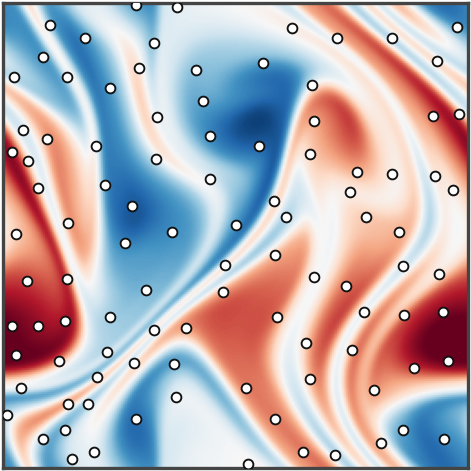
\includegraphics[width=2.9cm]{pipeline_panels/les_place}};
\node[anchor=north] at (15.5,12.20) {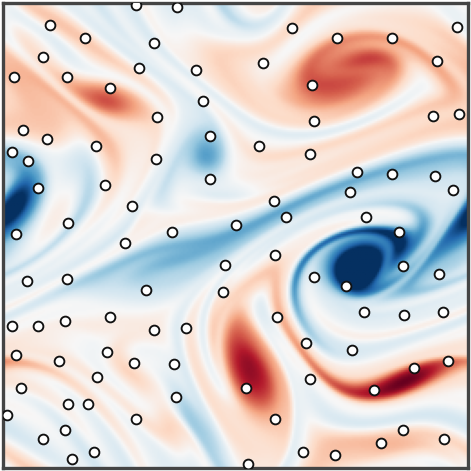
\includegraphics[width=2.9cm]{pipeline_panels/dns_measure}};
\node[anchor=north] at (20.6,12.20) {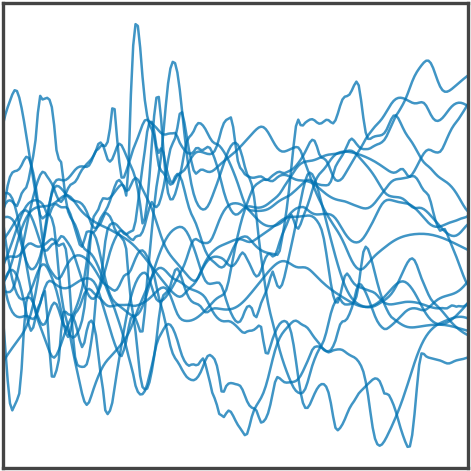
\includegraphics[width=2.7cm]{pipeline_panels/series}};
\node[el, anchor=north, text width=3.2cm, align=center] at (10.4,9.05)
  {low-cost LES\\ QR-pivot on a POD basis};
\node[el, anchor=north, text width=3.2cm, align=center] at (15.5,9.05)
  {real flow (DNS stand-in)\\ read $u,v$ at those $K$};
\node[el, anchor=north, text width=2.9cm, align=center] at (20.6,9.05)
  {$K=100$ streams\\ the only measured input};
\draw[ar] (11.95,10.7) -- (13.95,10.7) node[el, pos=0.5, above] {positions only};
\draw[ar] (17.05,10.7) -- (19.15,10.7) node[el, pos=0.5, above] {sample};

% ===================== BOTTOM BAND =====================
% ---- D: PI-CON operator (this work) ----
\draw[pnlb] (0.15,0.25) rectangle (13.55,7.55);
\node[anchor=north west, text=picon] at (0.35,7.40) {\PT{PI-CON operator (this work)}};

\node[io]  (sin)  at (1.45,5.45) {sensor stream\\ $[T,K,2]$};
\node[nd]  (rff)  at (3.75,5.45) {Fourier/RFF\\ + residual MLP};
\node[ndb] (att)  at (6.15,5.45) {token\\ self-attention};
\node[ndb] (cfc)  at (8.55,5.45) {CfC\\ causal scan $\Delta t$};
\node[io]  (qin)  at (1.45,1.75) {query\\ $(x,y,t_q)$};
\node[nd]  (tr)   at (3.75,1.75) {Fourier +\\ temporal anchor};
\node[ndb] (ca)   at (8.55,3.55) {cross-attention\\ isotropic distance bias};
\node[nd]  (fus)  at (11.15,3.55) {DeepONet\\ fusion $\langle b,\tau\rangle$};
\node[io]  (out)  at (12.75,1.75) {$(u,v,p)$};

\draw[ar] (sin) -- (rff);
\draw[ar] (rff) -- (att);
\draw[ar] (att) -- (cfc);
\draw[ar] (cfc.south) -- ++(0,-0.62) -| (ca.north) node[el, pos=0.28, above] {K,V};
\draw[ar] (qin) -- (tr);
\draw[ar] (tr.east) -- ++(0.6,0) |- (ca.west) node[el, pos=0.42, above] {Q};
\draw[ar] (ca) -- (fus);
\draw[ar] (fus.south) -- ++(0,-0.7) -| (out.north);

% ---- E: loss ----
\draw[pnl] (13.85,4.35) rectangle (23.35,7.55);
\node[anchor=north west, text=ink] at (14.05,7.40) {\PT{Sensor-only + PDE loss}};
\node[anchor=north west] at (14.15,6.80) {\scriptsize$
  \begin{aligned}
    \mathcal{L}_{\text{data}} &= \tfrac{1}{N}\textstyle\sum_i w_i
       \bigl(\hat{u}_{c_i}(\mathbf{x}_i,t_i;\theta)-u^{\text{obs}}_{c_i}\bigr)^{2}\\[2pt]
    \mathcal{L}_{\text{NS},u} &= \tfrac{1}{N_p}\textstyle\sum_j \mathcal{R}_u^{2},
      \qquad \mathcal{L}_{\text{NS},v}=\tfrac{1}{N_p}\textstyle\sum_j \mathcal{R}_v^{2}\\[2pt]
    \mathcal{R}_c &= \tfrac{\partial u}{\partial x}+\tfrac{\partial v}{\partial y},
      \qquad \mathcal{L}_{\text{cont}}=\tfrac{1}{N_p}\textstyle\sum_j \mathcal{R}_c^{2}
  \end{aligned}$};
\node[el, anchor=south west] at (14.15,4.50) {no full-field DNS target enters training};

% ---- F: weighting + optimiser ----
\draw[pnl] (13.85,0.25) rectangle (18.55,4.05);
\node[anchor=north west, text=ink] at (14.05,3.90) {\PT{Weighting + optimiser}};
\node[anchor=north west] at (14.05,3.32) {\tiny$
  \begin{aligned}
    \mathcal{L} &= \mathrm{GradNorm}\bigl(\mathcal{L}_{\text{data}},\mathcal{L}_{\text{NS},u},
       \mathcal{L}_{\text{NS},v},\mathcal{L}_{\text{cont}}\bigr)+\mathcal{L}_{\text{AL}}\\[2pt]
    \lambda &\leftarrow \min(\lambda+\beta\,\mathcal{C},\ \Lambda_{\max})\\[2pt]
    \theta^{\star} &= \arg\min_{\theta}\ \mathcal{L}(\theta)
  \end{aligned}$};
\node[el, anchor=south west] at (14.05,0.42) {SOAP + Schedule-Free};

% ---- G: output + offline evaluation ----
\draw[pnl] (18.85,0.25) rectangle (23.35,4.05);
\node[anchor=north west, text=ink] at (19.05,3.90) {\PT{Output and offline check}};
\node[anchor=north] at (20.15,3.30) {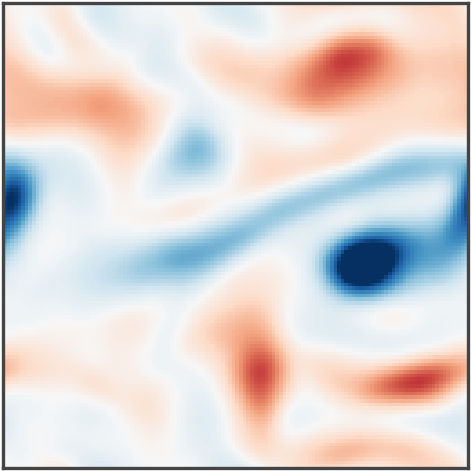
\includegraphics[width=1.85cm]{pipeline_panels/recon}};
\node[anchor=north] at (22.15,3.30) {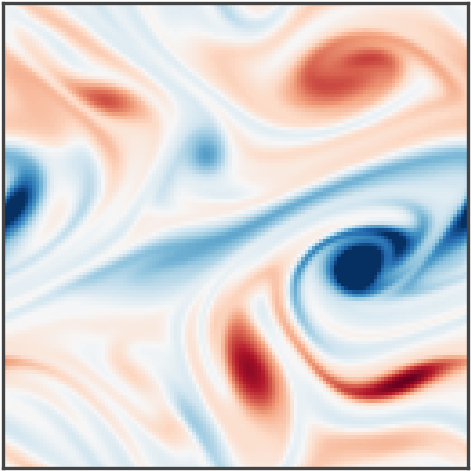
\includegraphics[width=1.85cm]{pipeline_panels/offline_ref}};
\node[el, anchor=north] at (20.15,1.32) {PI-CON};
\node[el, anchor=north] at (22.15,1.32) {DNS reference};
\node[el, anchor=south west, text width=4.2cm] at (19.05,0.35)
  {the DNS full field is used here only to score the result, never to train it};

% ===================== INTER-PANEL ARROWS =====================
\draw[gar] (3.9,7.95) -- (3.9,6.05);
\node[el, anchor=west, text=mute] at (4.05,7.05) {automatic differentiation};
\draw[gar] (20.6,7.95) -- (20.6,7.75) -- (0.85,7.75) -- (0.85,6.05);
\draw[gar] (13.55,5.95) -- (13.85,5.95);
\draw[gar] (16.2,4.35) -- (16.2,4.05);
\draw[gar] (13.55,1.75) -- (18.85,1.75) node[el, pos=0.12, above] {};
\draw[dar] (14.2,3.2) -- (13.1,3.2) -- (13.1,4.6) -- (12.2,4.6);
\node[el, anchor=south east, text=mute] at (14.1,3.25) {update $\theta$};

\end{tikzpicture}%
}%
\pdfpagewidth=\wd0
\pdfpageheight=\dimexpr\ht0+\dp0\relax
\hoffset=-1in \voffset=-1in
\shipout\box0
\end{document}
